\chapter{Materiais e Métodos}

Neste capítulo são descritos os procedimentos e materiais adotados no trabalho. Inicialmente, tem-se uma breve caracterização dos projetos selecionados nas organizações citadas na seção 3.4 inerente ao capítulo sobre metodologia. Posteriormente, são descritas todas as ferramentas utilizadas para desenvolvimento, gerenciamento e coleta de dados. Por fim, são apontadas as atividades executadas neste estudo de acordo com o procedimento técnico pesquisa-ação.

\section{Projetos selecionados na CGDF}

Pelo fato de o presente trabalho propor um \textit{framework} que reúne as práticas complementares e fundamentais da verificação de \textit{software} (testes e inspeções), bem como conceitos da VBSE, procurou-se selecionar produtos que possuem impacto significativo na missão da CGDF e que não possuíam tais práticas sendo utilizadas no seu processo de desenvolvimento.

\subsection{Portal da Transparência do Distrito Federal}

O primeiro produto selecionado foi o Portal da Transparência do Distrito Federal (www.transparencia.df.gov.br). Esta é uma ferramenta de participação da sociedade no controle das ações do Governo. Dentre as informações disponibilizadas pelo portal, destacam-se informações sobre a contabilidade do Governo do Distrito Federal, tais como: instrumentos de planejamento, receitas públicas arrecadadas pelo Governo, despesas públicas realizadas pelo Estado, licitações dos órgãos do Governo do Distrito Federal e remuneração dos servidores.

O Portal da Transparência do Distrito Federal já se encontra em sua terceira versão. De acordo com a CGDF, a reformulação do Portal, culminando em sua terceira versão, fez com que os acessos aumentassem em cerca de 34\% em dezembro de 2016 e janeiro de 2017 em relação ao mesmo período no ano passado. A quantidade de usuários únicos no site, nesse intervalo, passou de 174.232 para 234.653 de acordo com o último levantamento.

A terceira versão do Portal foi concebida de forma a facilitar a navegação do usuário, bem como a compreensão dos dados disponibilizados. Adicionalmente, procurou-se desenvolver uma solução escalável, de forma que os dados pudessem ser utilizados por outros sistemas.

Desde o início da concepção arquitetural da terceira versão do Portal foram adotadas tecnologias modernas no âmbito do desenvolvimento de aplicações \textit{web}. Basicamente, adotou-se o \textit{framework AngularJS} para elaboração da aplicação cliente e o \textit{Spring Framework}, desenvolvido em linguagem Java, para construção da API \textit{REST (Representational State Transfer)} que é utilizada como \textit{backend}. A seguir, tem-se a figura \ref{fig:portalInicio}, que exibe a página inicial do Portal e a figura \ref{fig:arquiteturaPortal}, que exibe um esquema da arquitetura do Portal.

\begin{figure}[h]
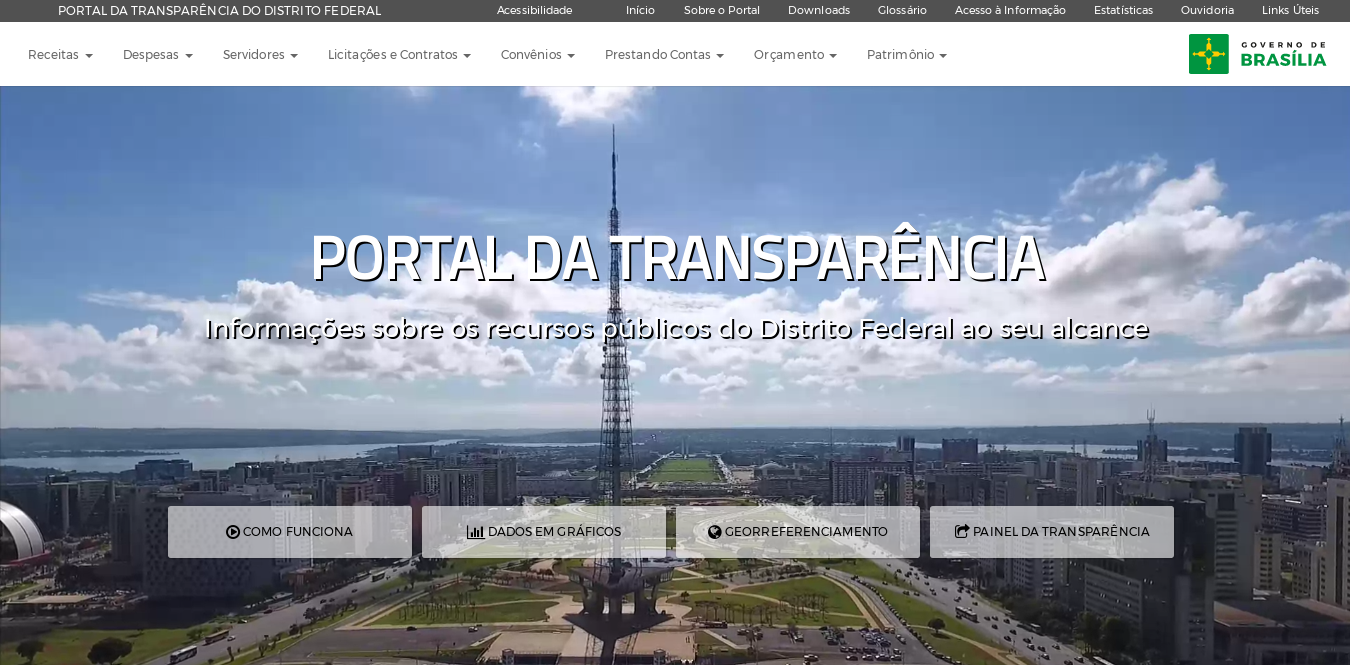
\includegraphics[width=\textwidth]{figuras/portalTransparencia.png}
\caption{Página inicial - Portal da Transparência do Distrito Federal}
\label{fig:portalInicio}
\end{figure}

\begin{figure}[h]
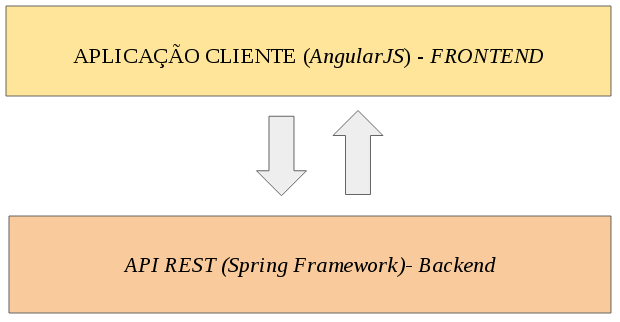
\includegraphics[width=\textwidth]{figuras/arquiteturaPortal.png}
\caption{Esquema Arquitetural - Portal da Transparência do Distrito Federal}
\label{fig:arquiteturaPortal}
\end{figure}

O Portal passa por constantes evoluções. Todos os dias dados são atualizados e novas funcionalidades são incorporadas em uma periodicidade de 3 semanas, tempo de duração de uma \textit{sprint} no processo de desenvolvimento da COTEC. 

A partir de uma coleta inicial de métricas, o Portal apresentou índice de manutenibilidade médio igual a 55 no código constituinte da camada de \textit{backend}. A cobertura de código era 0\%, devido à inexistência de uma suíte de testes unitários. Adicionalmente, realizando um levantamento dos relatórios de falhas reportadas pela área de negócio acerca das \textit{sprints} passadas, foi possível identificar um número médio de falhas igual a 5 a cada implantação em produção. Assim, percebeu-se a importância de utilizar concisamente práticas da verificação de \textit{software} para melhorar a qualidade do Portal.

\subsection{Sistema de Ouvidoria do Distrito Federal}

O segundo produto selecionado foi o Sistema de Ouvidoria do Distrito Federal (www.ouv.df.gov.br). A Ouvidoria é um espaço que organiza a comunicação entre o cidadão e o governo, favorecendo a participação popular, a transparência e o aperfeiçoamento da prestação dos serviços públicos.

Como parte da estrutura da CGDF, existe a Subcontroladoria denominada Ouvidoria-Geral do DF. Esta é responsável pela coordenação dos trabalhos das Ouvidorias Especializadas - localizadas em cada órgão do Governo do Distrito Federal.

O sistema de ouvidoria também passou por uma reformulação, sendo que já se encontra em sua segunda versão. Dentre as melhorias realizadas na navegação, foram incluídas novas funcionalidades que fornecem maior transparência ao cidadão durante o atendimento de sua manifestação.

Assim como no Portal da Transparência, durante a concepção arquitetural da segunda versão do sistema de ouvidoria foram adotadas tecnologias modernas para o desenvolvimento. A camada de apresentação também utiliza o \textit{framework AngularJS} e a camada \textit{backend} foi construída utlizando a linguagem \textit{CSharp} seguindo as diretrizes do estilo arquitetural MVC (\textit{Model, View, Controller}) e também, do estilo de desenvolvimento DDD (\textit{Domain Driven Design}). Posteriormente, a equipe do projeto optou por refatorar a camada de \textit{backend}, passando a utilizar \textit{Web API}.

O DDD, por sua vez, é uma abordagem que se alinha concisamente às ideias apresentadas pela VBSE, pois basicamente, um dos aspectos mais destacados nesta abordagem é que o código produzido deve estar bem alinhado ao negócio. Este conceito, se utilizado corretamente, favorece a reutilização pois os blocos de construção facilitam o aproveitamento de um mesmo conceito de domínio ou um mesmo código em vários lugares \cite{ddd}. Adicionalmente, com um modelo bem feito e organizado, as diversas partes de um sistema interagem sem que haja muita dependência entre os módulos ou classes de objetos de conceitos distintos, acarretando em um quadro mínimo de acoplamento.

Com relação ao projeto da Ouvidoria, o cenário relativo à implementação de testes unitários era idêntico ao do Portal da Transparência, ou seja, cobertura de código em 0\%. No âmbito do número médio de falhas reportadas pela área de negócio, o projeto da Ouvidoria possuía cerca de 4 falhas reportadas ao final de cada \textit{sprint} (falhas reportadas a cada implantação em produção). O código, contudo, apresentava um índice de manutenibilidade médio igual a 65.

Embora tenham sido feitas boas escolhas quanto às tecnologias e arquitetura, o sistema de ouvidoria também necessitava de um controle de qualidade mais rigoroso, visto que assim como o Portal, também passa por constantes evoluções. A figura \ref{fig:inicioOuvdf} exibe a página inicial do Sistema de Ouvidoria do Distrito Federal.

\begin{figure}[h]
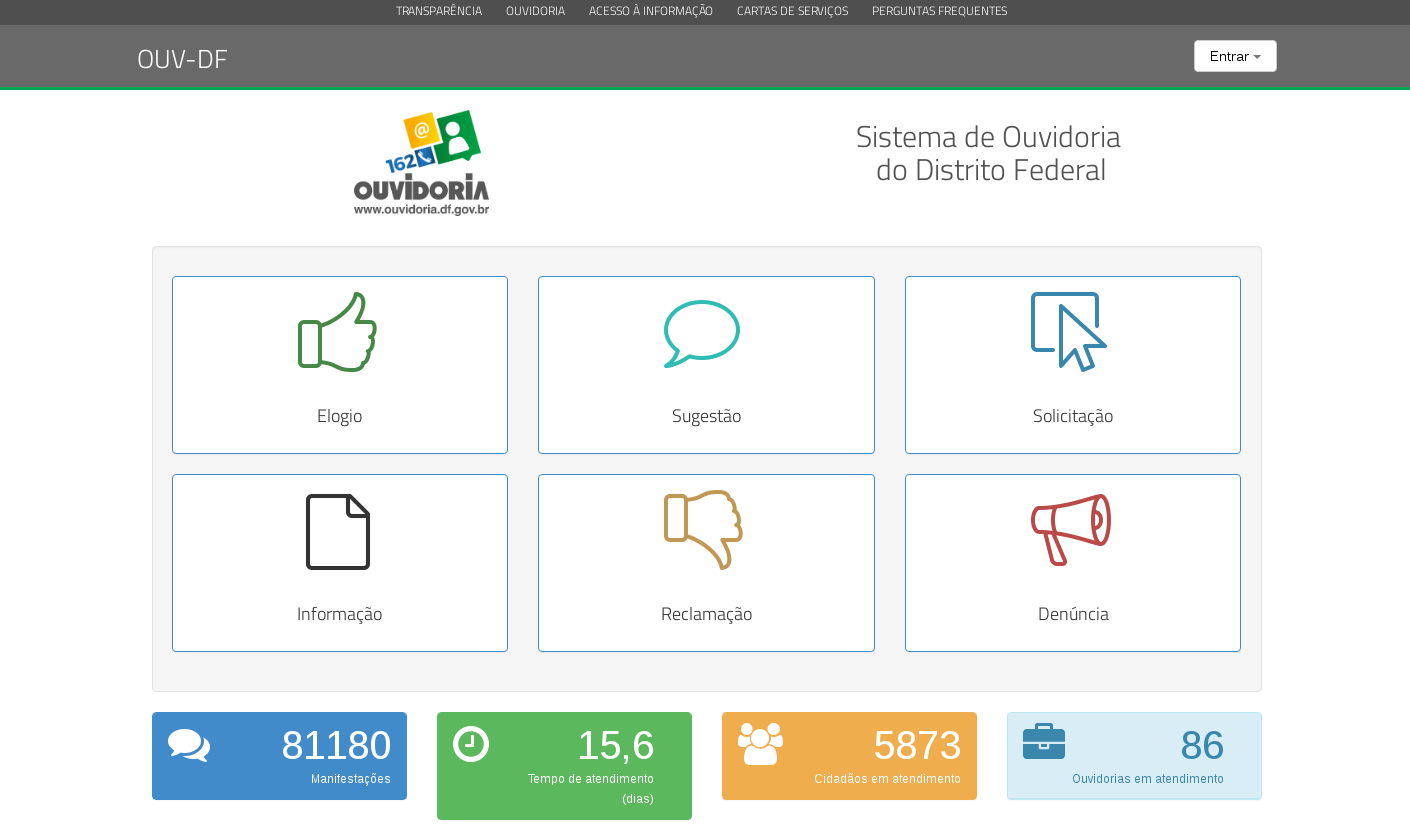
\includegraphics[width=\textwidth]{figuras/sistemaOuvidoria.png}
\caption{Página inicial - Sistema de Ouvidoria do Distrito Federal}
\label{fig:inicioOuvdf}
\end{figure}

\clearpage

\subsection{Sistema de Correição - SICOR}

Interna à CGDF existe a SUCOR (Subcontroladoria de Correição Administrativa). A SUCOR é uma das áreas que alicerçam a atuação da CGDF e tem como finalidade prevenir e apurar irregularidades no âmbito da Administração Pública, por meio da instauração e condução de procedimentos correcionais. Adicionalmente, exerce o papel de coordenação e supervisão das atividades correcionais dos órgãos e entidades do Governo do Distrito Federal.

Para o acordo de resultados de 2017, foi estabelecida a criação de um sistema para automatizar algumas atividades do fluxo de trabalho da SUCOR. Assim sendo, iniciou-se o projeto de desenvolvimento do SICOR.

Para desenvolvimento do sistema, a equipe de tecnologia optou por adotar a linguagem de programação \textit{Ruby} juntamente com o apoio do \textit{framework} \textit{Rails}. Quanto à arquitetura, o SICOR possui organização similar ao Portal, portando a camada de \textit{frontend} utilizando o \textit{framework AngularJS} e a camada de \textit{backend} como uma API \textit{REST}, desenvolvida em \textit{Ruby}.

A seleção deste projeto denota o desejo compartilhado entre a alta administração de TI e a área de negócio em se obter um produto sendo construído com qualidade desde o início. Adicionalmente, as práticas propostas pela VBSE, integrantes do \textit{framework} concebido neste trabalho, apresentam-se como essenciais para o êxito do projto. Desde o início o planejamento do projeto foi realizado com base nos itens mais críticos considerados pela área de negócio, tais como trilhas de auditorias, sigilo das informações e criptografia das informações trafegadas pela aplicação.

No capítulo 6 será possível contemplar os dados obtidos a partir do uso do \textit{framework} de avaliação da qualidade de código no projeto de desenvolvimento do SICOR.

\clearpage

\section{Projeto selecionado no Laboratório Fábrica de \textit{Software}}

\subsection{Sistema de Perícia Médica}

O Laboratório Fábrica de \textit{Software} possui atualmente uma parceria com uma instituição privada que, por motivos de políticas de sigilo, não terá sua identidade revelada neste trabalho. Contudo, a mesma será tratada como Instituição X.

A Instituição X é uma empresa que promove processos seletivos e aplica diversos tipos de exames no Brasil. Determinados processos seletivos organizados pela empresa necessitam de uma etapa adicional para a realização da perícia médica nos candidatos classificados para as fases posteriores. Atualmente, todo este processo é manual, envolvendo o preenchimento de fichas e um exaustivo trabalho para passar todos estes dados para o meio digital.

Tendo em vista esta oportunidade de negócio, a Instituição X solicitou o desenvolvimento de um sistema para automatizar o registro e compilação dos dados inerentes à perícia médica ao Laboratório Fábrica de \textit{Software}.

A solução proposta pelo Laboratório Fábrica de \textit{Software} envolve a elaboração de duas aplicações que funcionam de forma conjunta. Há uma aplicação \textit{web}, sendo desenvolvida em linguagem de programação \textit{CSharp}, seguindo o estilo arquitetural MVC. Nesta aplicação, a área de negócio pode montar fichas personalizadas de perícia médica para os diversos editais que são publicados. Adicionalmente, a aplicação \textit{web} recebe todos os dados enviados pela segunda aplicação, que é \textit{mobile} e esta foi projetada para ser utilizada nos locais de realização da perícia médica. A aplicação \textit{mobile} também está sendo desenvolvida em linguagem \textit{CSharp} e também segue as diretrizes do estilo arquitetural MVC.

A equipe de desenvolvimento do sistema de perícia médica também relatou a necessidade que possuíam de implementar um controle mais rigoroso da qualidade. O índice de manutenibilidade médio obtido a partir da primeira coleta foi igual a 55 e o número médio de falhas reportados pela área de negócio ao final de cada \textit{sprint} era igual a 5. Adicionalmente, a equipe também mencionou dificuldades na elaboração de testes unitários para a aplicação \textit{mobile}. Assim, o projeto caracterizou-se como uma excelente oportunidade para aplicação do \textit{framework} proposto por este trabalho.

\clearpage

\section{Ferramentas para Desenvolvimento e Coleta de Dados}

No contexto da CGDF, para o desenvolvimento do Portal da Transparência, utiliza-se a IDE (\textit{Integrated Development Environment}) \textit{Intellij}.

A IDE \textit{Intellij} fornece suporte nativo para as tecnologias utilizadas no desenvolvimento do Portal. Adicionalmente, possui compatibilidade com diversos \textit{plugins}, dentre eles, o \textit{Metrics Reloaded}, o \textit{plugin} adotado neste estudo para coleta das métricas de código fonte do projeto Portal.

Por fim, é válido destacar que a IDE \textit{Intellij} já possui integração nativa com a biblioteca JaCoCo (\textit{Java Code Coverage}), que fornece uma análise detalhada acerca da cobertura do código a partir da coloração apresentada no código fonte. As cores apresentadas pela biblioteca possuem significados específicos:

\begin{itemize}
	\item \textbf{Linhas Verdes:} Indicam que a suíte de testes cobriu o referido trecho de código tanto pela abordagem de \textit{statement coverage} quanto pela abordagem de \textit{branch coverage}.

	\item \textbf{Linhas Amarelas:} Indicam que a suíte de testes cobriu parcialmente o referido trecho de código. Neste cenário, faz-se necessária a construção de mais um método de teste para exercitar o trecho faltante.

	\item \textbf{Linhas Vermelhas:} Indicam que a suíte de testes não foi capaz de exercitar o referido trecho de código. Faz-se necessária a construção de métodos de teste para fazê-lo.
\end{itemize}

As figuras \ref{fig:metricsReloaded} e \ref{fig:jacoco} exibem, respectivamente, a tela de customização de métricas do \textit{Metrics Reloaded Plugin} e um trecho de código analisado pela biblioteca JaCoCo após execução da suíte de testes.

\begin{figure}[h]
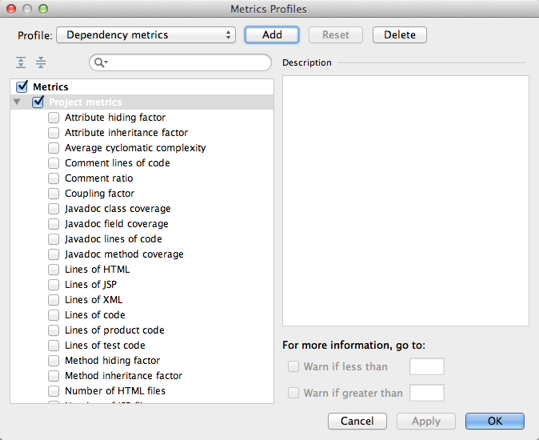
\includegraphics[width=\textwidth]{figuras/metricsReloaded.png}
\caption{Tela de Customização de Métricas - \textit{Metrics Reloaded Plugin}}
\label{fig:metricsReloaded}
\end{figure}

\begin{figure}[h]
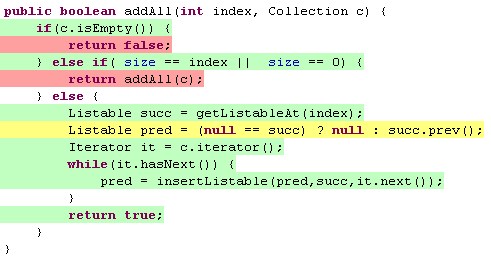
\includegraphics[width=\textwidth]{figuras/jacoco.png}
\caption{Análise de Cobertura de Código - Jacoco}
\label{fig:jacoco}
\end{figure}

\clearpage

Com relação ao Sistema de Ouvidoria do Distrito Federal e ao Sistema de Perícia Médica, pelo fato de serem sistemas desenvolvidos em linguagem \textit{CSharp}, utiliza-se a IDE \textit{Visual Studio}.

A IDE \textit{Visual Studio}, em sua versão \textit{Ultimate}, possui suporte para análise de cobertura de código e coleta de métricas.

De forma semelhante à biblioteca JaCoCo, a IDE \textit{Visual Studio} exibe uma coloração específica para a análise de cobertura após execução da suíte de testes. Uma coloração azul claro é exibida nos trechos de código exercitados de forma efetiva pela suíte de testes (\textit{statement coverage} e \textit{branch coverage}). As linhas de código que apresentam uma coloração vermelha expressam insuficiência de métodos de teste na suíte para exercitá-las.

Por fim, com relação ao projeto SICOR, adotou-se o \textit{Simplecov} como ferramenta de análise de cobertura e a ferramenta \textit{Metric fu} para coleta de métricas de código fonte.

As figuras \ref{fig:coberturaVS} e \ref{fig:metricasVS} exibem, respectivamente, uma análise de cobertura de código feita pela IDE \textit{Visual Studio} após execução de uma suíte de testes e o resultado da coleta de métricas.

\begin{figure}[h]
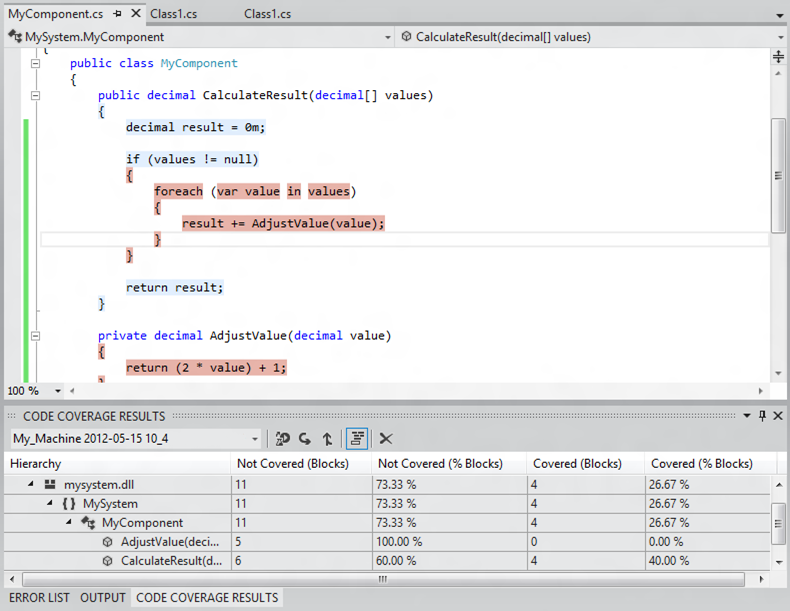
\includegraphics[width=\textwidth]{figuras/codeCoverageVS.png}
\caption{Análise de Cobertura de Código - \textit{Visual Studio}}
\label{fig:coberturaVS}
\end{figure}

\begin{figure}[h]
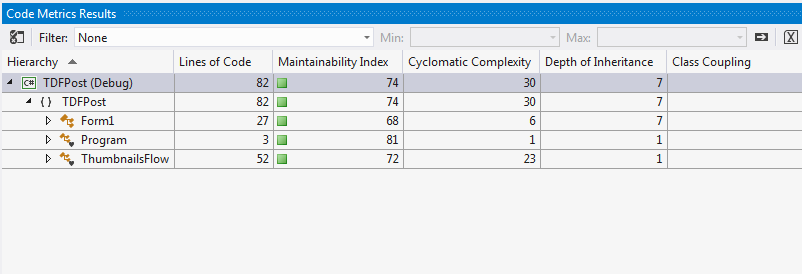
\includegraphics[width=\textwidth]{figuras/metricsVS.png}
\caption{Coleta de Métricas - \textit{Visual Studio}}
\label{fig:metricasVS}
\end{figure}

\section{Ferramenta para Gerenciamento e Inspeções de Código}

Tanto no contexto da CGDF como também do Laboratório Fábrica de \textit{Software}, utiliza-se a ferramenta de gerenciamento TFS (\textit{Team Foundation Server}). A ferramenta já apresenta suporte para gerenciamento de projetos que adotam metodologias ágeis, especificamente o \textit{Scrum}. A figura \ref{fig:tfs} exibe a página inicial da ferramenta.

\begin{figure}[h]
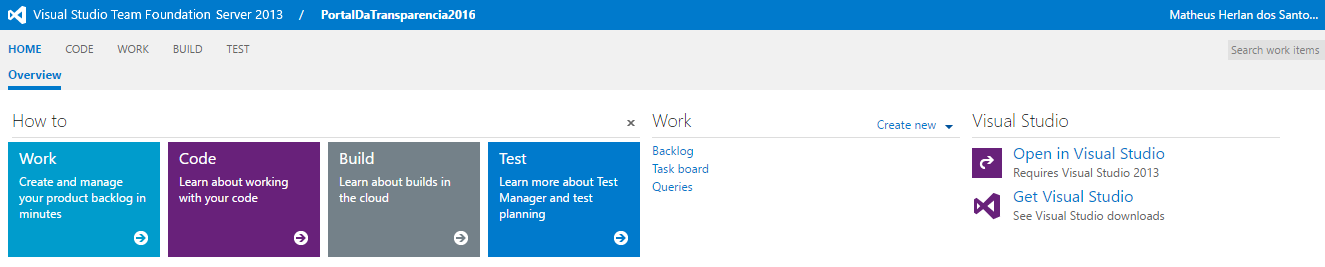
\includegraphics[width=\textwidth]{figuras/tfs.png}
\caption{Página inicial - \textit{Team Foundation Server}}
\label{fig:tfs}
\end{figure}

É válido ressaltar que a ferramenta TFS possui suporte para a realização de \textit{Pull Requests}, a forma encontrada neste estudo para que as inspeções fossem devidamente realizadas. O fluxo básico para realização das inspeções, tanto na CGDF como também no Laboratório Fábrica de \textit{Software}, apresenta os seguintes passos:

\begin{enumerate}
	\item O desenvolvedor, após finalizar a implementação da sua funcionalidade, submeterá um \textit{Pull Request} da sua \textit{branch} para a \textit{branch approval}. Durante este processo, o desenvolvedor deverá delegar esta inspeção a qualquer outro desenvolvedor membro do projeto.

	\item O desenvolvedor que for designado para efetuar a inspeção deverá aplicar os \textit{checklists} propostos pelo \textit{framework} concebido neste estudo e efetuar os devidos apontamentos para o desenvolvedor que submeteu o \textit{Pull Request}.

	\item Após correções e ajustes, caso necessário, o desenvolvedor que realizou a inspeção deverá efetuar a mesclagem do código na \textit{branch approval}.

	\item Ao final da \textit{sprint}, todo o código da \textit{branch approval} será mesclado na \textit{branch} de homologação para entrega das funcionalidades desenvolvidas na \textit{sprint} à área de negócio.

	\item Após homologação da \textit{release} entregue, será feita a contabilização do número de falhas inerentes às novas funcionalidades entregues, caso sejam notadas. Por fim, ocorrerá mesclagem do código na \textit{branch} master.
\end{enumerate}

\section{Ferramenta para Coleta do Índice de Satisfação dos Desenvolvedores}

Para coletar a percepção dos desenvolvedores com relação ao uso do \textit{framework} proposto neste estudo, foi elaborado um formulário por meio da ferramenta \textit{Google Forms}. Basicamente, foram colocadas as questões e alternativas, segundo escala \textit{Likert}, já apresentados no capítulo sobre metodologia. A figura \ref{fig:questionario} exibe a página inicial do formulário eletrônico.

\begin{figure}[h]
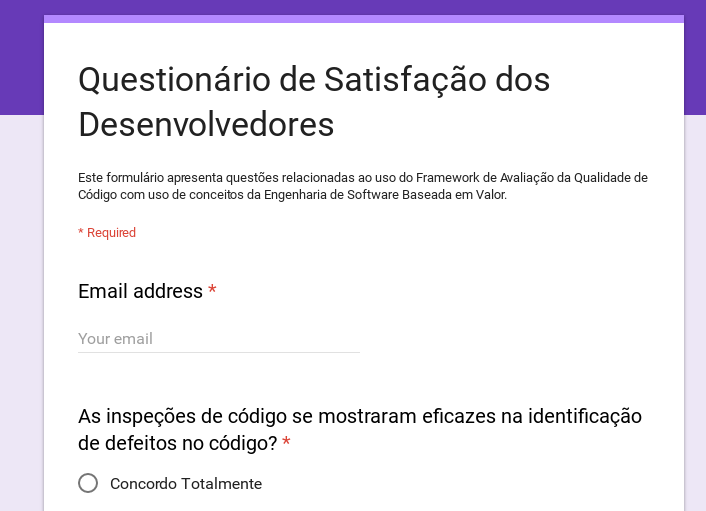
\includegraphics[width=\textwidth]{figuras/questionario.png}
\caption{Formulário Eletrônico - Índice de Satisfação dos Desenvolvedores}
\label{fig:questionario}
\end{figure}

\section{Planejamento da Aplicação do \textit{Framework}}

Inicialmente, planejou-se um período de treinamento nas organizações. Na CGDF, a cultura de implementação de testes unitários e realização de inspeções ainda estava em seu estágio inicial. Portanto, foi preparado um treinamento contemplando modelos de implementação de testes unitários para todas as tecnologias utilizadas no desenvolvimento dos projetos selecionados. Adicionalmente, explicitou-se mais conceitos inerentes às inspeções para que os \textit{checklists} propostos pelo \textit{framework} aplicado neste estudo ficassem mais elucidativos.

No Laboratório Fábrica de \textit{Software}, de forma semelhante, também foi promovido um treinamento inicial. Contudo, o foco deste treinamento esteve centralizado na implementação de testes unitários para aplicações \textit{mobile}, uma das principais dificuldades relatadas pela equipe de desenvolvimento do projeto da perícia médica.

Como o \textit{framework} utilizado neste estudo já se caracteriza como um processo alinhado às atividades e práticas do \textit{Scrum}, os ciclos de pesquisa-ação, basicamente, são as \textit{sprints} dos projetos de desenvolvimento. É válido notar que ao final de cada \textit{sprint}, serão realizadas coletas de percepções de forma a aprimorar as atividades propostas pelo \textit{framework}. A seguir, tem-se a figura \ref{fig:planejamento1}, que exibe o planejamento inicial dos ciclos de coleta de dados.

\begin{figure}[h]
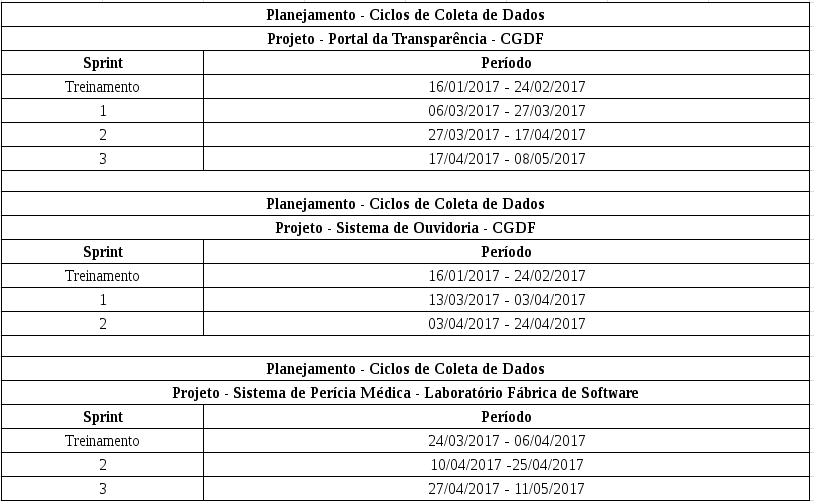
\includegraphics[width=\textwidth]{figuras/planejamento.png}
\caption{Planejamento inicial - Ciclos de Coleta de Dados}
\label{fig:planejamento1}
\end{figure}

Ao longo da execução dos ciclos de coleta de dados alguns ajustes foram necessários. Na CGDF, por causa do surgimento de uma demanda emergencial, a execução do projeto do Sistema de Ouvidoria foi temporariamente suspensa e assim, não houve tempo hábil para coletar os dados da segunda \textit{sprint} do mesmo.

O projeto do Portal, devido também à demanda emergencial da CGDF, teve sua execução suspensa temporariamente. As equipes de desenvolvimento destes projetos foram realocadas para atendimento da demanda. Adicionalmente, como o projeto de desenvolvimento do SICOR surgiu em tempo oportuno, resolveu-se adotar o mesmo como caso para aplicação do \textit{framework} proposto neste trabalho.

Com relação ao Laboratório Fábrica de \textit{Software} também foi necessário efetuar um ajuste no planejamento, visto que a equipe apresentou dificuldades em realizar as inspeções após treinamento, comprometendo o que havia sido planejado inicialmente. Assim, optou-se por fazer mais uma reunião para retratar como a coleta deveria ser feita e o planejamento passou a contemplar as \textit{sprints} subsequentes.

A figura \ref{fig:planejamento2} exibe o planejamento final deste trabalho.

\begin{figure}[h]
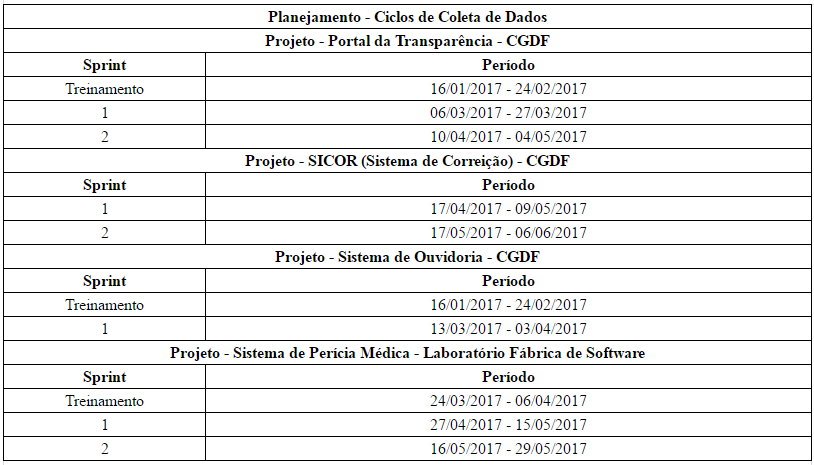
\includegraphics[width=\textwidth]{figuras/planejamento2.png}
\caption{Planejamento final - Ciclos de Coleta de Dados}
\label{fig:planejamento2}
\end{figure}

\section{Diagnóstico Inicial dos Projetos}

Na CGDF, como nenhum projeto era adepto de uma cultura centralizada em verificação, antes da aplicação do \textit{framework}, não havia implementação de testes unitários e também, realização de inspeções. Em muitas ocasiões, modificações efetuadas em um determinado componente do código fonte alterava o comportamento de outro componente. Este aspecto era percebido posteriormente pelos desenvolvedores durante atividades de \textit{debug}.

No Laboratório Fábrica de Software já ocorria implementação de testes unitários, porém, somente as classes do pacote \textit{controller} possuíam testes implementados. A partir de uma rápida inspeção nos códigos de teste, identificou-se a necessidade de refatorar trechos de código repetidos, bem como implementar mais cenários de testes de forma que o código fonte dos componentes sob teste fosse concisamente exercitado.

\section{Restrições existentes na Coleta de Dados}

Com base nas tecnologias utilizadas para construção dos sistemas, ferramentas existentes para coleta de métricas e disponibilidade das equipes para executar as atividades de verificação, foram delimitados escopos de coletas.

No projeto do Portal, foi acordado realização de inspeções e implementação de testes unitários tanto para o código da camada de \textit{frontend} quanto da camada \textit{backend}. Com relação à análise do índice de manutenibilidade, somente a camada de \textit{backend} foi utilizada. A camada de \textit{frontend}, por se feita em \textit{Java Script}, não possui um suporte conciso em termos de ferramentas para realizar a análise desta métrica.

Quanto ao projeto da Ouvidoria, foi acordado realização de inspeções e implementação de testes somente para a camada de \textit{backend}. A equipe do projeto, por não possuir experiência em verificação, considerou melhor aplicar o \textit{framework} inicialmente desta maneira. Contudo, a equipe do projeto pretende futuramente incluir a camada de \textit{frontend} nas análises.

Por fim, no Laboratório Fábrica de Software, optou-se também por efetuar as inspeções e implementação de testes unitários somente na camada de \textit{backend}.

É válido ressaltar que tanto no projeto da Ouvidoria quanto no projeto da Perícia Médica, foram acordadas inspeções rápidas do código da camada de \textit{frontend} antes da mesclagem nas \textit{branches} oficiais. Porém, seus resultados não foram considerados formalmente para os fins da análise efetuada neste trabalho.

\clearpage